% Template for ICASSP-2021 paper; to be used with:
%          spconf.sty  - ICASSP/ICIP LaTeX style file, and
%          IEEEbib.bst - IEEE bibliography style file.
% --------------------------------------------------------------------------
\documentclass{article}
\usepackage{spconf,amsmath,graphicx}
\graphicspath{ {./images/} } % set path to images

% Example definitions.
% --------------------
\def\x{{\mathbf x}}
\def\L{{\cal L}}

% Title.
% ------
\title{Fine-tuning MLLM for multimodal question answering}
%
% Single address.
% ---------------
\name{Sara Boukili \qquad Philippe Gélinas \qquad Antoine Reid}
%
% For example:
% ------------
\address{Université Laval\\
	Département d'informatique et de génie logiciel\\
	IFT-4030 Apprentissage automatique pour le traitement du signal}

\begin{document}
%\ninept
%
\maketitle
%
\begin{abstract}
The abstract should appear at the top of the left-hand column of text, about
0.5 inch (12 mm) below the title area and no more than 3.125 inches (80 mm) in
length.  Leave a 0.5 inch (12 mm) space between the end of the abstract and the
beginning of the main text.  The abstract should contain about 100 to 150
words, and should be identical to the abstract text submitted electronically
along with the paper cover sheet.  All manuscripts must be in English, printed
in black ink.
\end{abstract}
%
\begin{keywords}
One, two, three, four, five
\end{keywords}
%
\section{Introduction}
\label{sec:intro}
LLM fine-tuning is a very active research topic and new methods are constantly being proposed. However, fine-tuning LLMs is computationaly expensive and most current techniques are prohibitively expensive for consumer hardware. We aim to fine-tune a multimodal LLM (MLLM) for a multiple-choice question answering task with consumer-grade hardware. Therefore, we limit ourselves to GPUs with no more than 15GB of VRAM and LLMs with no more than 8b parameters. We use the ScienceQA dataset as a benchmark to evaluate different fine-tuning techniques and models. We focus mainly on parameter-efficient fine-tuning as they allow training on consumer hardware. We also explored prompt-tuning which can be an alternative to fine-tuning. We briefly explored using RAG instead of fine-tuning but found this method to be unsuitable for our task.

\section{Literature review}
\label{sec:litreview}

LoRA (Low-Rank Adaptation) is a fine-tuning technique for LLMs introduced by \cite{lora}. It deviates from regular fine-tuning by freezing the original model weights and by updating a separate set of weights which are then added to the original weights. In regular fine-tuning an entire weight update matrix ($\Delta W$) is combined with the pre-trained weights. LoRA separates $\Delta W$ into 2 low-rank matrices that approximate it. This method significantly reduces the number of trainable parameters. Along with the reduced computational load this brings, it can also help prevent overfitting. Compared to other adapter based fine-tuning techniques, LoRA does not introduce increased inference latency during inference. The downside of LoRA is that it introduces a new hyperparameter, $r$, which must be optimized. This hyperparameter represents the inner dimension of the low-rank matrices.\par

QLoRA \cite{qlora} is a modification of LoRA that introduces increased memory efficiency due to storing weight parameters with 4-bit precision. To achieve this, the authors used 3 concepts : a new data type, 4-bit NormalFloat, which is theoretically optimal for normally distributed data, double quantization of quantization constants to increase the memory efficiency, and paged optimizers to handle memory spikes. \cite{qlora} observed performance levels similar to those of LoRA. Another LoRa variant is DoRA \cite{dora}, which is supposed to outperform LoRa for fine-tuning LLMs for various tasks, including ours, which relates to image-text understanding. DoRA decomposes the weights of a pre-trained model into magnitude and direction components. DoRA can be applied in the same way as LoRA, and allows its variants like QDoRA.\par

ProMoT (Prompt Tuning with Model Tuning) \cite{valizadehaslani2022twostagefinetuningnovelstrategy} addresses the challenge of language models becoming overly specialized during fine-tuning, which can reduce their general capabilities. It uses a two-stage approach that offloads format learning to additional parameters through prompt tuning, allowing for comparable performance on the fine-tuned task while preserving or even enhancing general in-context learning abilities. This flexibility in managing various output formats and task types is particularly beneficial for the diverse question types in the ScienceQA dataset.\par

An extensive review of RAG \cite{ragreview} has found that RAGs can help address hallucination and outdated knowledge problems. The advantage of RAG is that they allow for continuous knowledge update to the model and can allow an LLM to incorporate knowledge outside of the training domain. RAG are not always better than fine-tuning, especially for tasks which require specific data formats as inputs and a response in a particular style.\par



\section{Method}
\label{sec:method}

\subsection{Parameter-Efficient Fine-Tuning (PEFT)}
For this section, we will test PEFT methods on two models: LLaVA-1.5\cite{liu2023llava} and Idefics2\cite{idefics2}. These
two models were chosen because they possess a number of parameters small enough to be suitable for training on consumer-grade GPUs, while still being able to handle multimodal inputs (image and text) which is required for the task at hand. Idefics2 contains roughly 8b parameters while LLaVA-1.5 contains roughly 7b parameters. Idefics2 was created by the HuggingFace team and was shown to outperform much larger LLMs on several benchmarks. LLaVA-1.5 uses CLIP ViT-L/14 as a visual encoder and Vicuna (itself based on Llama) as the LLM decoder. During fine-tuning we keep the vision encoder (the part of the model that tokenizes the images) frozen.\par

Traditional fine-tuning is far too costly for consumer hardware because of the sheer numer of parameters to train. For example, Idefics2 contains roughly 8.4 billion parameters, which would require about 16GB of VRAM to store. When fine-tuning with Adam optimizer, this would be even greater because the optimizer stores 3 copies of the weights. PEFT methods make fine-tuning larger NLP models much more accessible by only training a small subset of model parameters while keeping the vast majority of the base model's parameters frozen.\par

LoRA significantly reduces the number of trainable parameters by approximating a weight update matrix with two low-rank matrices. LoRA only applies to linear layers of the model. LoRA can reduce the number of trainable parameters by 10,000 times. When using LoRA fine-tuning with a rank of 8 for Idefics2, we reduced the number of trainable parameters from 8.4b to 23.3m. We are training less than 0.1\,\% of the total model parameters! LoRA methods introduce two hyperparameters to set: the rank of the adapter matrices $r$ and the layers which are actually fine-tuned.\par

Despite the important reduction in trainable parameters LoRA offers, it can still be too costly to fine-tune an LLM with 8b parameters on a consumer GPU. This is because the base model, even when frozen, requires too much storage space. To alleviate this problem, we utilize quantization. Generally, the model parameters of an LLM are stored in 16 or 32-bit formats. Quantization compresses these parameters into 4-bit which significantly reduces the memory footprint. Although quantization introduces a loss of information, the impact of the quantization error is minimized by the fine-tuning (during training the model learns and incorporates the quantization error). QLoRA combines quantization and LoRA and is the first PEFT method we will use. It is important to understand that only the frozen parameters are stored in 4-bit, the LoRA adapter layers and the Adam optimizer are not quantized.

LoRA was found to have much a much different learning behavior than full fine-tuning. Furthermore, LoRA performs worse than full fine-tuning in certain situations. DoRA corrects these shortcomings by decomposing the pretrained weights into their magnitude and direction. LoRA is then applied to the directional component, while the magnitude component is trained as is. The second PEFT method we utilize is a quantized version of DoRA.

We will fine-tune both models with PEFT methods on a train set of the ScienceQA dataset and then evaluate the performance of the model on the test set. Given that there are a varying number of choices (between 2 and 5), we use accuracy as a performance metric.

\subsection{Prompt tuning}

\begin{table*}[t]
  \centering
  \begin{tabular}{lrrr}
    \hline
    Model & Trainable parameters & Training time & Accuracy (\%)\\ 
    \hline
    Idefics2 QLoRA (r=8) & 23,326,720 & 6h 18min & 89.14\\ 
    Idefics2 QLoRA (r=4) & 11,663,360 & 4h 52min & 88.20\\ 
    Idefics2 QLoRA last 50 layers (r=8) & 4,734,976 & 1h & 77.00\\
    Idefics2 DoRA (r=6) & 19,033,856 & 10h 13min & 89.54\\
    LLaVA QLoRA (r=6) & 15,876,096 & 10h 20min & 83.28\\
    LLaVA DoRA (r=6) & 17,309,696 & - & -\\
    Prompt-tuning & - & 4 days & 79.44\\
    \hline
  \end{tabular}
  \caption{Accuracy of models on test dataset}
  \label{tab:model_performance}
\end{table*}

\section{Experiments}
\label{sec:experiments}

\subsection{ScienceQA dataset}
As mentioned, we will use the ScienceQA dataset. The ScienceQA dataset contains 21\,208 multimodal multiple-choice questions collected from primary and high school curricula. The questions are separated into 3 subjects: natural science, language science, and social science. Roughly 49\,\% of the questions have an image context, 48\,\% have a text context, and 31\,\% have both. An interesting aspect of the ScienceQA dataset is that most question contain lectures (84\,\%) and detailed explanations (91\,\%) that help answer the question. The dataset has already been split into train, test, and validation sets on HuggingFace. The train set contains 12\,726 observations, whereas the test and validation sets each contain 4\,241 observations. Figure \ref{fig:example_q} shows a typical question from the dataset.

\begin{figure}
  \centering
  \centerline{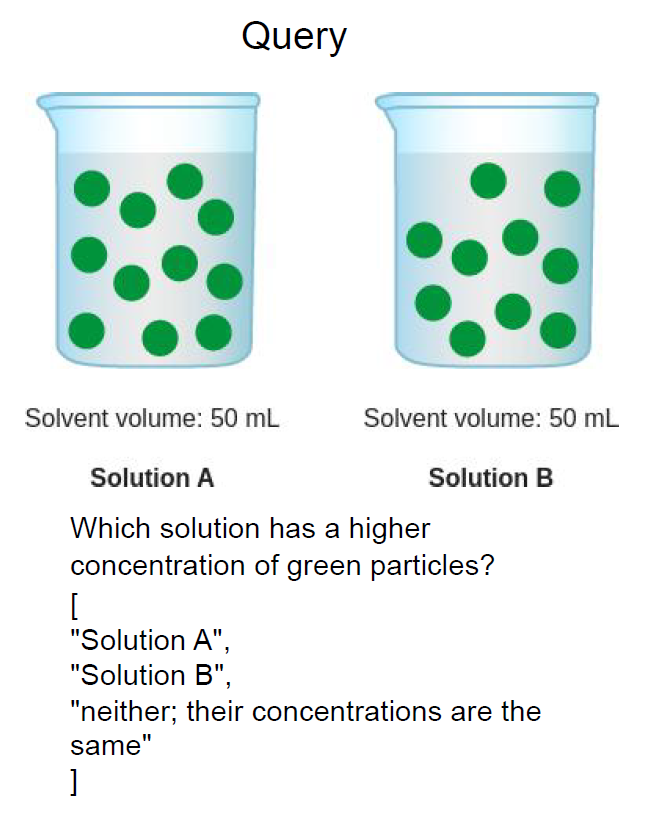
\includegraphics[scale=0.5]{example_question.png}}
  \caption{Example question from the ScienceQA dataset}
  \label{fig:example_q}
\end{figure}

\subsection{Training details}

\subsection{Results}

Table \ref{tab:model_performance} presents the results of our various models and fine-tuning techniques.


Not suprising Idefics2 beat LLaVA-1.5 because it accepts greater image resolution, has beaten LLaVA-1.5 in benchmarks, and is more recent. 


\section{Conclusion}
\label{sec:conclusion}



% Below is an example of how to insert images. Delete the ``\vspace'' line,
% uncomment the preceding line ``\centerline...'' and replace ``imageX.ps''
% with a suitable PostScript file name.
% -------------------------------------------------------------------------
\begin{figure}[htb]

\begin{minipage}[b]{1.0\linewidth}
  \centering
  % \centerline{\includegraphics[width=8.5cm]{image1}}
%  \vspace{2.0cm}
  \centerline{(a) Result 1}\medskip
\end{minipage}
%
\begin{minipage}[b]{.48\linewidth}
  \centering
  % \centerline{\includegraphics[width=4.0cm]{image3}}
%  \vspace{1.5cm}
  \centerline{(b) Results 3}\medskip
\end{minipage}
\hfill
\begin{minipage}[b]{0.48\linewidth}
  \centering
  % \centerline{\includegraphics[width=4.0cm]{image4}}
%  \vspace{1.5cm}
  \centerline{(c) Result 4}\medskip
\end{minipage}
%
\caption{Example of placing a figure with experimental results.}
\label{fig:res}
%
\end{figure}


% To start a new column (but not a new page) and help balance the last-page
% column length use \vfill\pagebreak.
% -------------------------------------------------------------------------
%\vfill
%\pagebreak


\vfill\pagebreak


% References should be produced using the bibtex program from suitable
% BiBTeX files (here: strings, refs, manuals). The IEEEbib.bst bibliography
% style file from IEEE produces unsorted bibliography list.
% -------------------------------------------------------------------------
\bibliographystyle{IEEEbib}
\bibliography{refs}

\end{document}
